
% LaTeX Beamer file automatically generated from DocOnce
% https://github.com/hplgit/doconce

%-------------------- begin beamer-specific preamble ----------------------

\documentclass{beamer}

\usetheme{red_plain}
\usecolortheme{default}

% turn off the almost invisible, yet disturbing, navigation symbols:
\setbeamertemplate{navigation symbols}{}

% Examples on customization:
%\usecolortheme[named=RawSienna]{structure}
%\usetheme[height=7mm]{Rochester}
%\setbeamerfont{frametitle}{family=\rmfamily,shape=\itshape}
%\setbeamertemplate{items}[ball]
%\setbeamertemplate{blocks}[rounded][shadow=true]
%\useoutertheme{infolines}
%
%\usefonttheme{}
%\useinntertheme{}
%
%\setbeameroption{show notes}
%\setbeameroption{show notes on second screen=right}

% fine for B/W printing:
%\usecolortheme{seahorse}

\usepackage{pgf,pgfarrows,pgfnodes,pgfautomata,pgfheaps,pgfshade}
\usepackage{graphicx}
\usepackage{epsfig}
\usepackage{relsize}

\usepackage{fancybox}  % make sure fancybox is loaded before fancyvrb

\usepackage{fancyvrb}
%\usepackage{minted} % requires pygments and latex -shell-escape filename
%\usepackage{anslistings}
%\usepackage{listingsutf8}

\usepackage{amsmath,amssymb,bm}
%\usepackage[latin1]{inputenc}
\usepackage[T1]{fontenc}
\usepackage[utf8]{inputenc}
\usepackage{colortbl}
\usepackage[english]{babel}
\usepackage{tikz}
\usepackage{framed}
% Use some nice templates
\beamertemplatetransparentcovereddynamic

% --- begin table of contents based on sections ---
% Delete this, if you do not want the table of contents to pop up at
% the beginning of each section:
% (Only section headings can enter the table of contents in Beamer
% slides generated from DocOnce source, while subsections are used
% for the title in ordinary slides.)
\AtBeginSection[]
{
  \begin{frame}<beamer>[plain]
  \frametitle{}
  %\frametitle{Outline}
  \tableofcontents[currentsection]
  \end{frame}
}
% --- end table of contents based on sections ---

% If you wish to uncover everything in a step-wise fashion, uncomment
% the following command:

%\beamerdefaultoverlayspecification{<+->}

\newcommand{\shortinlinecomment}[3]{\note{\textbf{#1}: #2}}
\newcommand{\longinlinecomment}[3]{\shortinlinecomment{#1}{#2}{#3}}

\definecolor{linkcolor}{rgb}{0,0,0.4}
\hypersetup{
    colorlinks=true,
    linkcolor=linkcolor,
    urlcolor=linkcolor,
    pdfmenubar=true,
    pdftoolbar=true,
    bookmarksdepth=3
    }
\setlength{\parskip}{0pt}  % {1em}

\newenvironment{doconceexercise}{}{}
\newcounter{doconceexercisecounter}
\newenvironment{doconce:movie}{}{}
\newcounter{doconce:movie:counter}

\newcommand{\subex}[1]{\noindent\textbf{#1}}  % for subexercises: a), b), etc

%-------------------- end beamer-specific preamble ----------------------

% Add user's preamble




% insert custom LaTeX commands...

\raggedbottom
\makeindex

%-------------------- end preamble ----------------------

\begin{document}

% endif for #ifdef PREAMBLE



% ------------------- main content ----------------------



% ----------------- title -------------------------

\title{Education for the future}

% ----------------- author(s) -------------------------

\author{Morten Hjorth-Jensen\inst{1,2}
\and
Hans Petter Langtangen\inst{3}
\and
Anders Malthe-Sørenssen\inst{1}}
\institute{Department of Physics, University of Oslo\inst{1}
\and
Department of Physics and Astronomy, Michigan State University, USA\inst{2}
\and
Department of Informatics, University of Oslo and Simula Research Laboratory\inst{3}}
% ----------------- end author(s) -------------------------

\date{September 2 2015, 
% <optional titlepage figure>
}

\begin{frame}[plain,fragile]
\titlepage
\end{frame}

\begin{frame}[plain,fragile]
\frametitle{How we perceive the role of education, present and future}

\begin{block}{}
The main topics of this talk are:

\begin{itemize}
\item \textbf{Research-based education}, from undergraduate studies to a PhD: \href{{http://www.mn.uio.no/fysikk/english/research/groups/computational/index.html}}{The Computational Physics group at the University of Oslo} as example

\item Future challenges and directions
\end{itemize}

\noindent
\end{block}
\end{frame}

\begin{frame}[plain,fragile]
\frametitle{The role of computations, from education to society}

\begin{block}{}

\textbf{Computations of almost all systems in science are central to our
basic understanding of nature and technological advances}.

The increase in computational power,
improved algorithms for solving problems in science as well as access
to high-performance facilities, allow researchers nowadays to study
complicated systems across many length and energy scales. Applications
span from studying quantum physical systems in nanotechnology and the
characteristics of new materials or subamotic physics at its smallest
length scale, to simulating galaxies and the evolution of the universe.

Simulations are key to understanding
cancer treatment and how the brain works,
predicting climate changes and this week's weather,
simulating natural disasters, semi-conductor devices,
quantum computers, as well as assessing risk in the insurance and
financial industry. 


\end{block}
\end{frame}

\begin{frame}[plain,fragile]
\frametitle{What do we mean with computing and computational science and physics?}

\begin{block}{}

\textbf{Computing means solving scientific problems using computers. It covers numerical as well as symbolic computing. Computing is also about developing an understanding of the scientific process by enhancing the algorithmic thinking when solving problems.}

And this  competence is about:

\begin{itemize}
\item derivation, verification, and implementation of algorithms

\item understanding what can go wrong with algorithms

\item overview of important, known algorithms

\item understanding how algorithms are used to solve complicated problems

\item reproducible science and ethics

\item algorithmic thinking for gaining deeper insights about scientific problems
\end{itemize}

\noindent
All these elements (and many more) aid students in maturing and gaining a better understanding of the scientific process.  
\end{block}
\end{frame}

\begin{frame}[plain,fragile]
\frametitle{Modeling and computations as a way to enhance algorithminc thinking}

\begin{block}{}

Algorithmic  thinking as a way to

\begin{itemize}
\item Enhance instruction based teaching

\item Introduce research-based teaching  from day one

\item Trigger further insights in math and other disciplines 

\item Validation and verification of scientific results, with the possibility to emphasize ethical aspects as well. Version control is central.

\item Good working practices from day one.
\end{itemize}

\noindent
\textbf{Algorithm} : A finite set of unambiguous instructions that, given some set of initial conditions, can be performed in a prescribed sequence to achieve a certain goal.
\end{block}
\end{frame}

\begin{frame}[plain,fragile]
\frametitle{Computing and research-based education}

\begin{block}{}
A computational approach allows us to introduce research concepts and engage students in research from \emph{day one}.
\end{block}
\begin{block}{How do we define it? }
It is coupled to a direct participation in actual research and builds upon established
knowledge and insights about scientific methods.
\end{block}
\end{frame}

\begin{frame}[plain,fragile]
\frametitle{Research-based education}

\begin{block}{What should the education contain? }
The standard situation we meet at an almost daily basis:

\begin{itemize}
\item Theory+experiment+simulation is almost the norm in research and industry

\item To be able to model complex systems with no simple answers. Solve real problems.

\item Emphasis on insight and understanding of fundamental principles and laws in the Sciences.

\item Be able to visualize, present, discuss, interpret and come with a critical analysis of the results, and develop a sound ethical attitude to own and other's work.
\end{itemize}

\noindent
Our education should reflect this. An example where this takes place is the \href{{http://www.mn.uio.no/fysikk/english/research/groups/computational/index.html}}{Computational Physics group at UiO}.  How did we implement the above visions? 
\end{block}
\end{frame}

\begin{frame}[plain,fragile]
\frametitle{\href{{http://www.mn.uio.no/fysikk/english/research/groups/computational/index.html}}{Computational Physics group at UiO}; implementing the vision}

\begin{block}{}
A particular strength of physics students is their ability to pose and
solve problems that combine physical insights with mathematical tools
and now also computational skills. This provides a unique combination
of applied and theoretical knowledge and skills. These features are invaluable 
for the development of multi-disciplinary educational and research programs. 
\end{block}
\end{frame}

\begin{frame}[plain,fragile]
\frametitle{Develop a social, scientific and learning environment}

\begin{block}{}
\begin{itemize}
\item The main aim is that students should realize their own potentials and creative power

\item The computational physics group includes bachelor, master of science and doctoral students

\item Project oriented work where students develop and mature their own ideas, with an individually tailored approach to each students

\item Office space with desktops to every student and large common room for recreational activities (meals, common lunches, gaming, watching movies etc etc)

\item Many students collaborate on similar  thesis topics and \href{{http://www.dn.no/talent/2014/06/12/Utdannelse/sommervikar-ble-toppforsker}}{publish in top scientific articles}
\end{itemize}

\noindent
\end{block}
\end{frame}

\begin{frame}[plain,fragile]
\frametitle{Developing a good learning environment}

\begin{block}{}
\begin{itemize}
\item Our students have made significant contributions to  the \href{{http://www.mn.uio.no/english/about/collaboration/cse/}}{Computing in Science Education}  (UiO education prize in 2011) by developing exercises and participating in educational projects at the MN faculty

\item Our students have also developed educational tools like \href{{http://www.mn.uio.no/fysikk/om/aktuelt/aktuelle-saker/2015/realfagsapper.html}}{tools and applications for understanding complicated physical problems} 

\item The students keep shaping and developing the scientific, social and pedagogical activities of the group

\item During the last ten years more than 60 students have finalized their master theses in computational physics and  almost 60\% have continued with PhD studies

\item Many students don't want to leave the group after finishing their studies
\end{itemize}

\noindent
\end{block}
\end{frame}

\begin{frame}[plain,fragile]
\frametitle{Investing in equipment for students}

\begin{block}{Using research funds for visualization tools }


% inline figure
\centerline{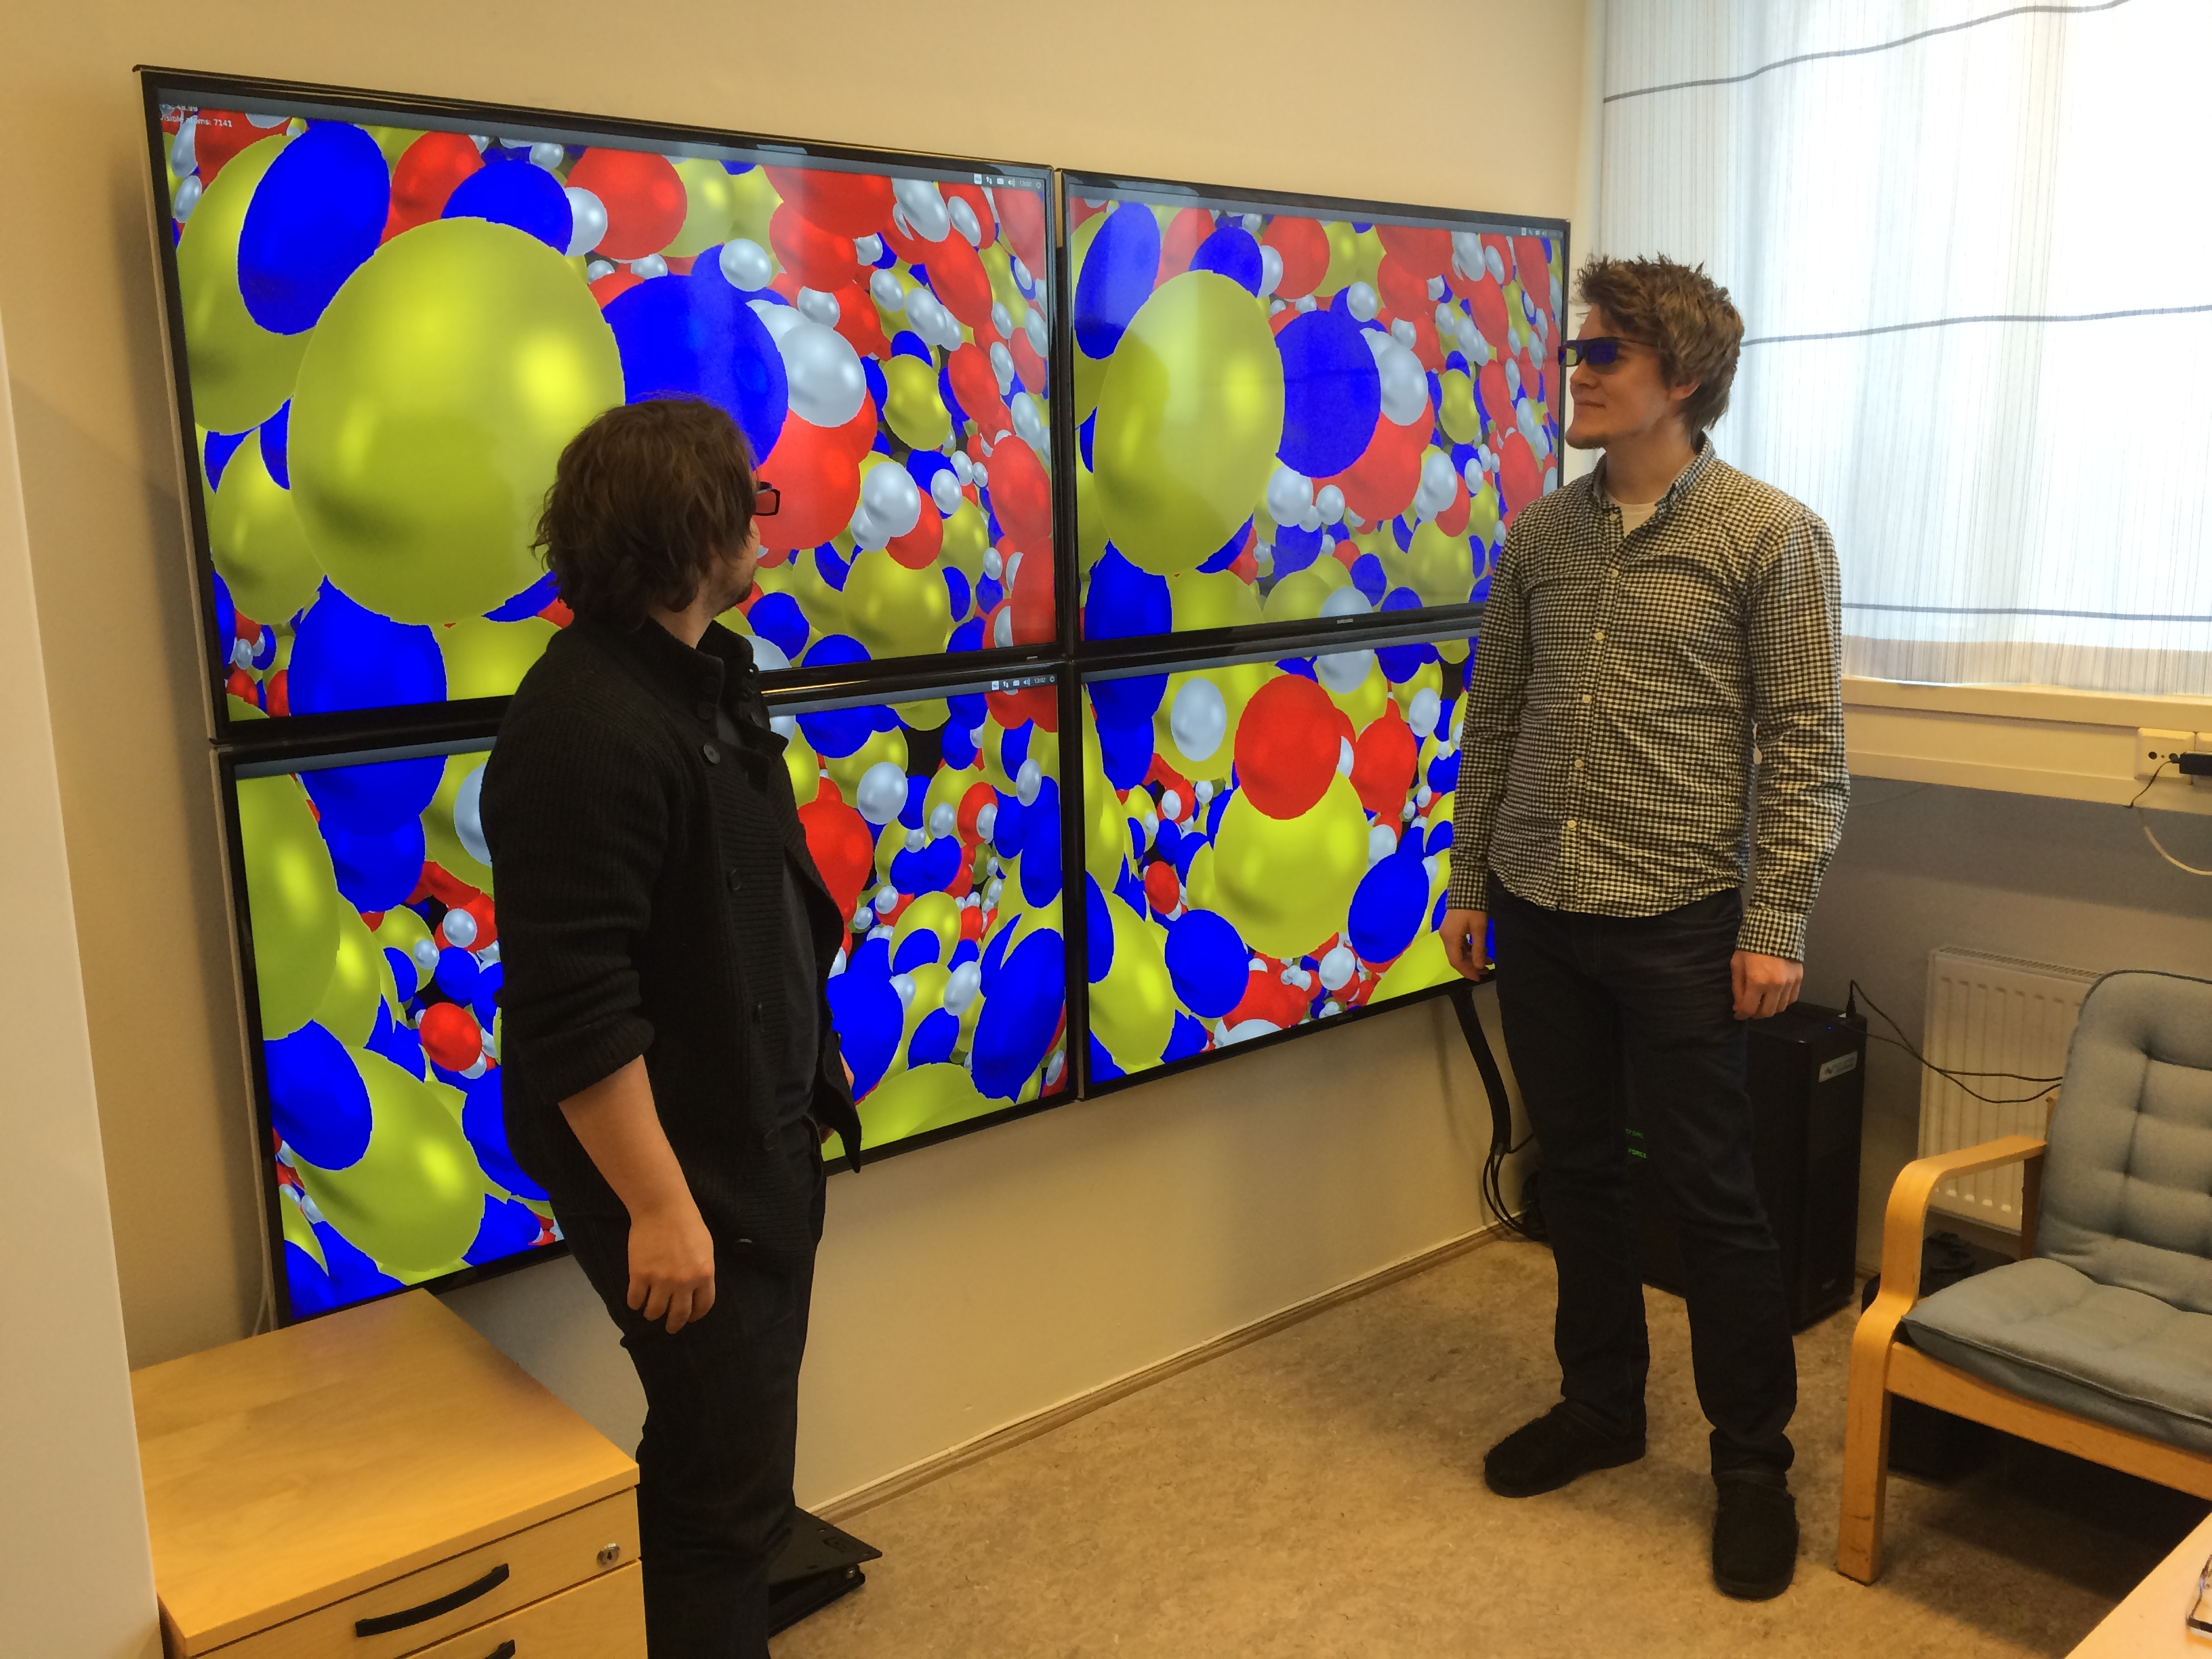
\includegraphics[width=0.7\linewidth]{fig-future/visualize.jpg}}



\end{block}
\end{frame}

\begin{frame}[plain,fragile]
\frametitle{Building a supercomputing cluster}

\begin{block}{We got (for free) the old supercomputer at UiO (TITAN) }


% inline figure
\centerline{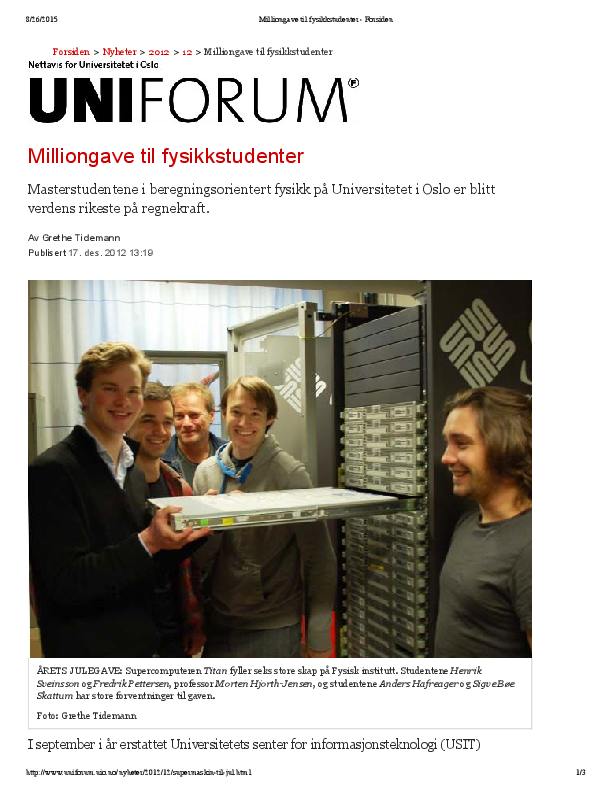
\includegraphics[width=0.7\linewidth]{fig-future/uniforum-0.png}}



\end{block}
\end{frame}

\begin{frame}[plain,fragile]
\frametitle{Undergraduate student publishes in PNAS}

\begin{block}{Using research funds for visualization tools }


% inline figure
\centerline{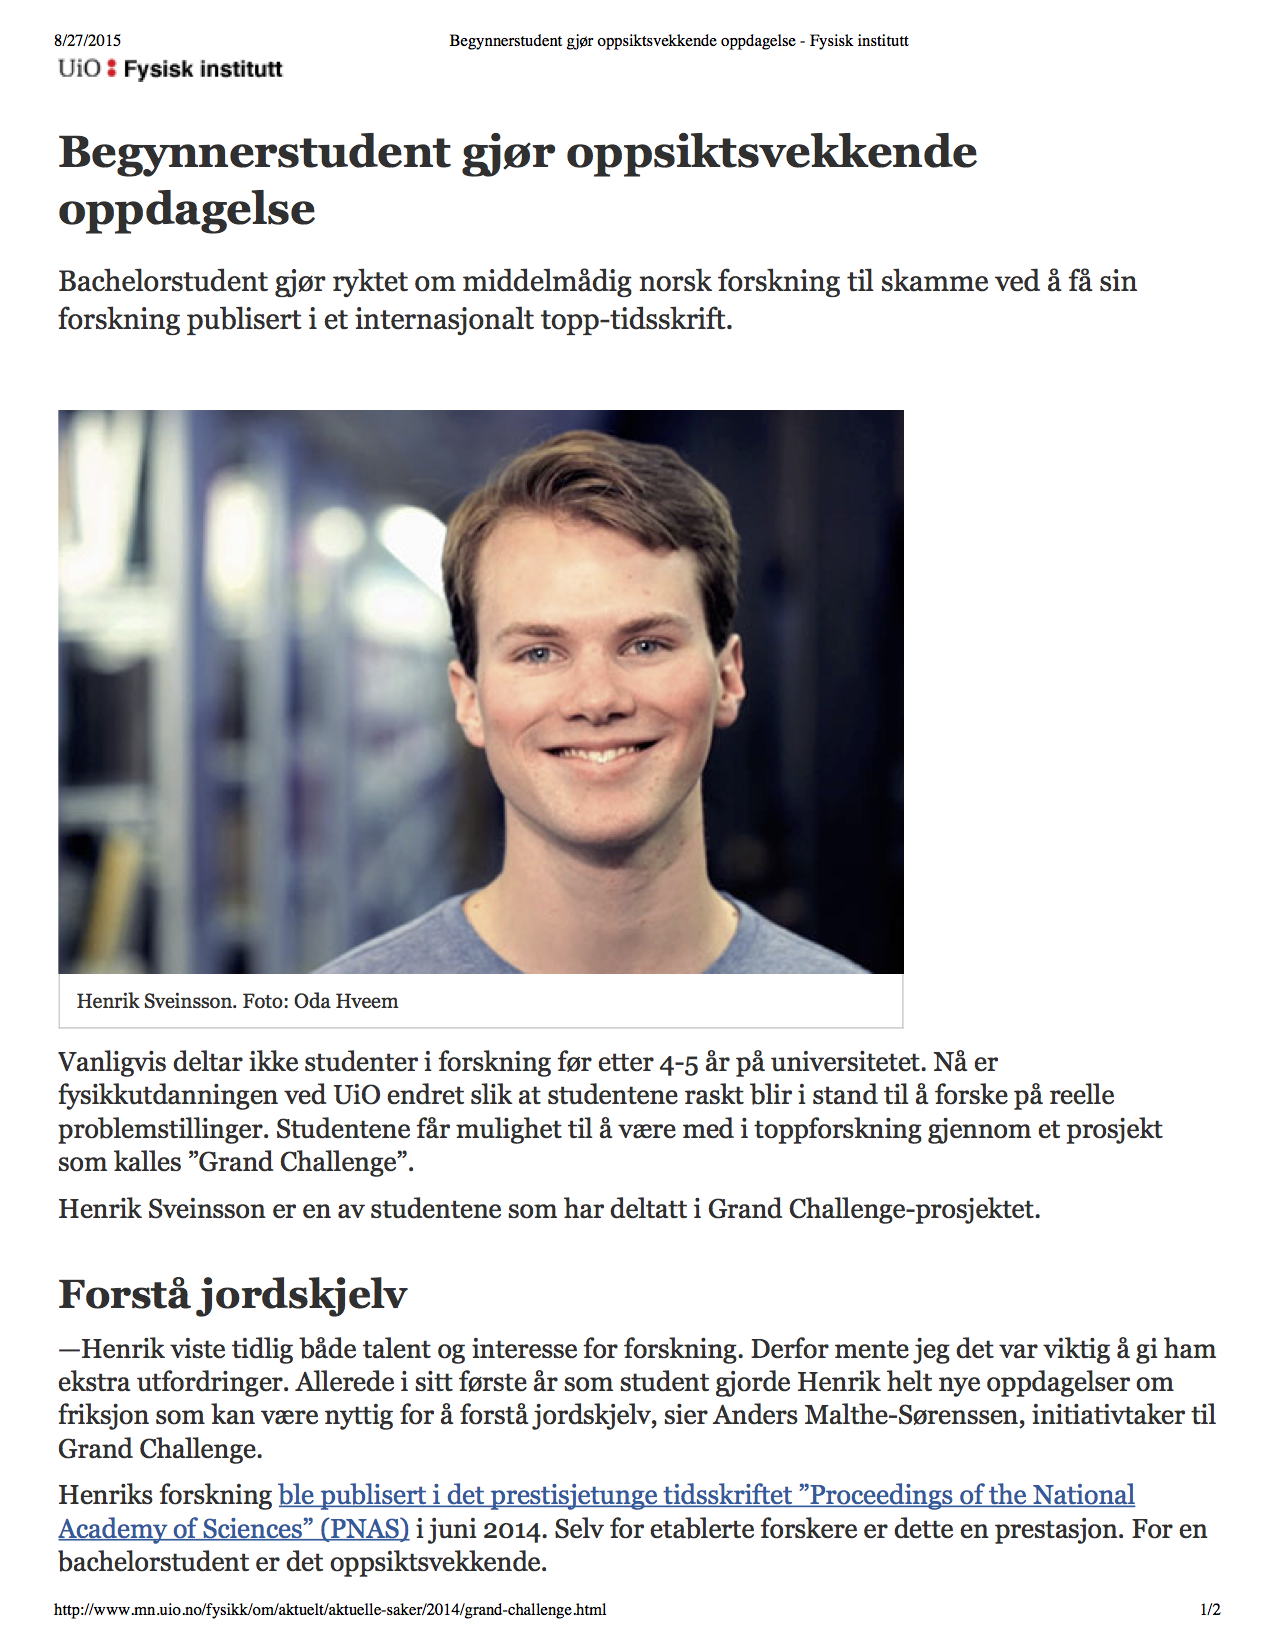
\includegraphics[width=0.7\linewidth]{fig-future/pnas.png}}



\end{block}
\end{frame}

\begin{frame}[plain,fragile]
\frametitle{The future: Multiscale modeling is the big open research question}

\begin{block}{}
Present and future problems, unlike traditional
science and engineering, involve complex systems with many distinct
physical processes. The wide open research topic of this century, both
in industry and at universities, is how to effectively couple
processes across different length and energy scales. Progress will
rely on a multi-disciplinary approach and therefore the  need for
multi-disciplinary educational and research programs.
\end{block}

\begin{block}{}
We need to foster candidates with the right
multi-disciplinary background and computational thinking for
understanding present and future simulation technologies and their challenges.
\end{block}
\end{frame}

\begin{frame}[plain,fragile]
\frametitle{Examples of large scale simulations}

\begin{block}{Fluid dynamical simulations central in air industry.  Typical university courses which are taught address the physics of the lower left corner.  }


% inline figure
\centerline{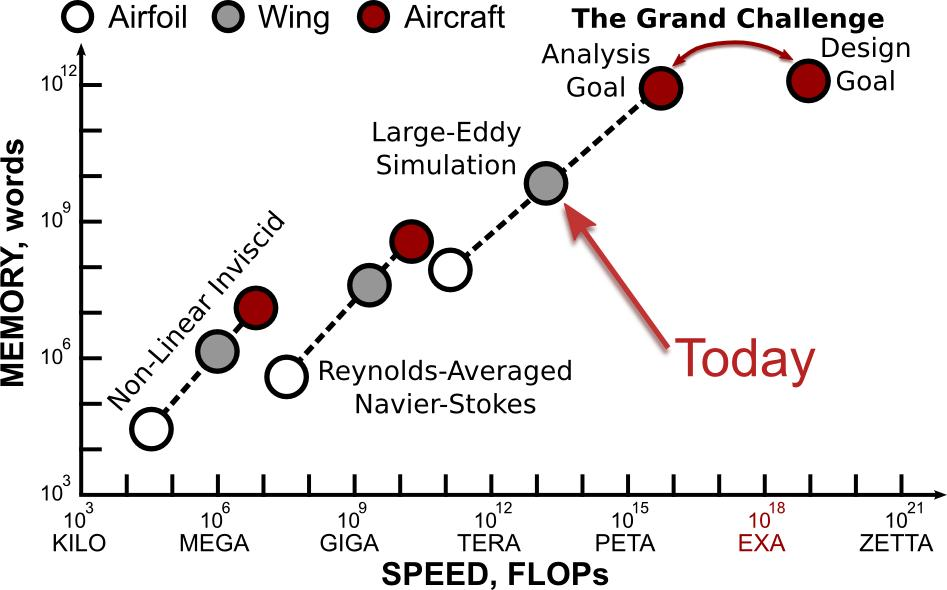
\includegraphics[width=0.6\linewidth]{fig-future/fig10.jpg}}


\end{block}
\end{frame}

\begin{frame}[plain,fragile]
\frametitle{Testing plane wings via massive numerical simulations}

\begin{block}{}
Fluid dynamical simulations central in air industry, wings tested.


% inline figure
\centerline{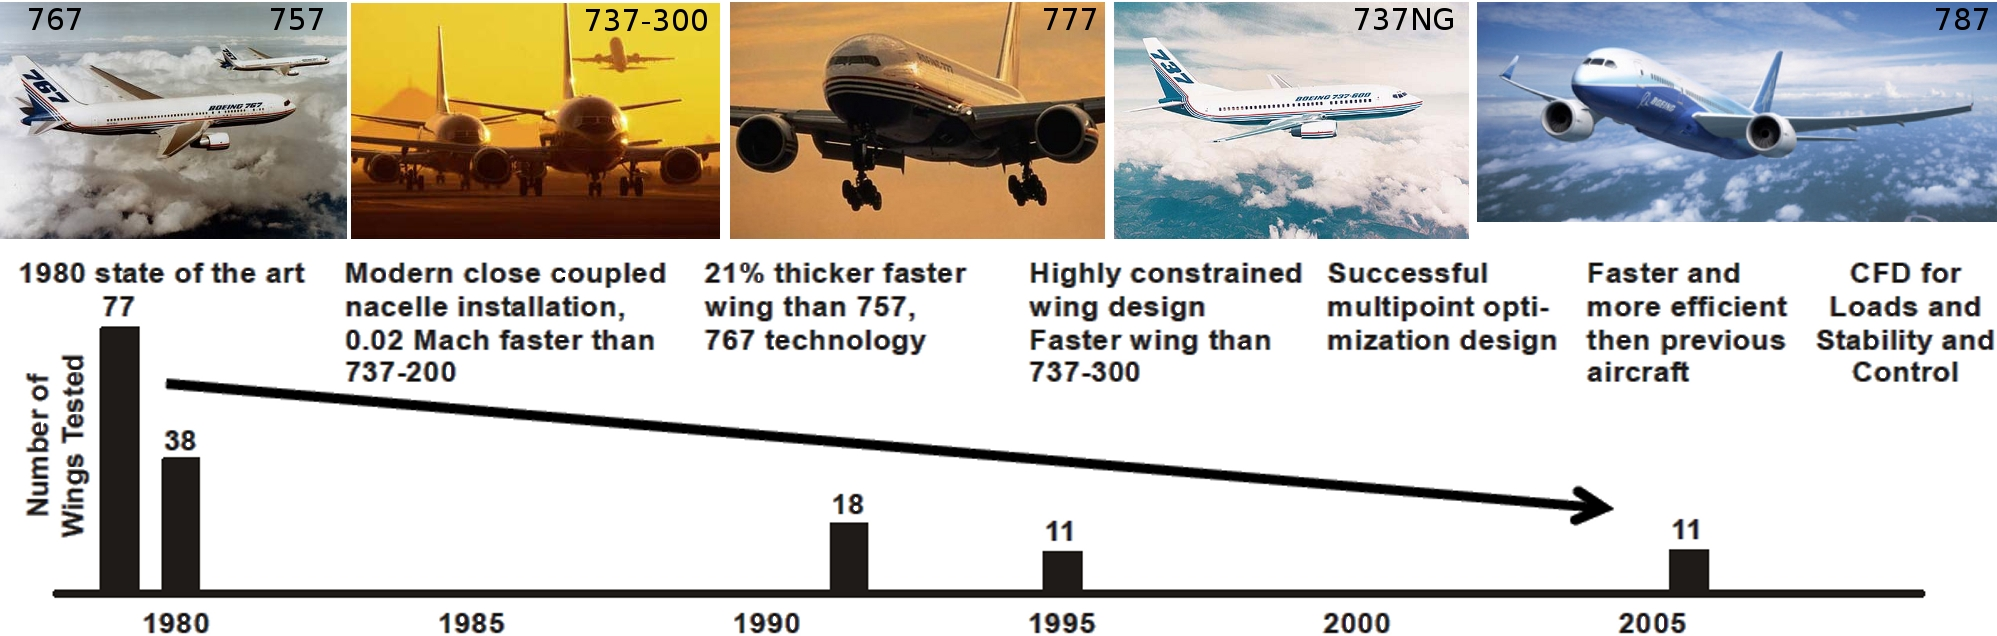
\includegraphics[width=1.0\linewidth]{fig-future/fig8.jpg}}


\end{block}
\end{frame}

\begin{frame}[plain,fragile]
\frametitle{The challenges for the future}

\begin{block}{}
We need to educate the next generation of 
science students with the knowledge, skills, and values needed to pose
and solve current and new scientific, technological and societal
challenges. 
\end{block}
\begin{block}{}
This will lay the foundation for cross-disciplinary
educational, research and innovation activities. It will contribute to building a common cross-disciplinary
approach to key strategic initiatives, with examples like \emph{Energy, Materials, Life Science, and Enabling Technologies}. 
\end{block}
\end{frame}

\begin{frame}[plain,fragile]
\frametitle{A new type of students}

\begin{block}{}
Candidates who are capable of modeling and understanding complicated
systems, are in short supply in society.  The
computational methods and approaches to scientific problems students learn
when working on their thesis projects are very similar to the methods
they will use in later stages of their careers.  To handle large
numerical projects demands structured thinking and good analytical
skills and a thorough understanding of the problems to be solved. This
knowledge makes the students unique on the labor market, a labor market which in the years to come will experience heavy automatization and massive loss of jobs.
\end{block}

\begin{block}{}
Computations (mastering and developing)  will play a central role in almost all aspects of scientific investigations and technological innovation
\end{block}
\end{frame}

\begin{frame}[plain,fragile]
\frametitle{What we should do: create the Department  for Computational Science}

\begin{block}{What we have and where we can arrive }
\begin{itemize}
\item UiO's strength in computational science (education and research) will play an important role in  determining new research and educational directions

\item Exploiting this strength has the potential to make UiO a center of excellence for scientific innovation
\end{itemize}

\noindent
\end{block}

\begin{block}{How to achieve it }
\begin{itemize}
\item Establish  a new center/department with focus on computational science and its applications to a wide range of fields (natural science, medicine, social sciences, humanities, applied research etc)

\item Hire ten (or more) young professors (age $< 40$) dedicated to innovative research and education where computations play a central role

\item Establish another ten professorships (or more) with  shared positions (position percentage  is flexible) between the  new department and the department of appartanence (physics, chemistry, etc etc).
\end{itemize}

\noindent
\end{block}

\textbf{The process must start now} in order not to loose momentum.
\end{frame}

\begin{frame}[plain,fragile]
\frametitle{The Computing in Science Education project, UiO educational prize in 2011}

\begin{block}{}
The insights, ideas and thoughts presented here, would have been impossible or difficult to gain without discussions, exchange of ideas and much more over many years with colleagues involved in the \href{{http://www.mn.uio.no/english/about/collaboration/cse/}}{Computing in Science Education} project at UiO. These dear friends and colleagues  are 
\begin{itemize}
\item Knut Mørken, Mathematics

\item Arnt Inge Vistnes, Physics

\item Oyvind Ryan, Mathematics

\item Solveig Kristensen, Dean of Education, MN faculty

\item Hanne Sølna, Director of studies MN faculty
\end{itemize}

\noindent
\end{block}
\end{frame}

\end{document}
